%
% hardware.tex
%
% Copyright (C) 2020 by SpaceLab.
%
% EPS 2.0 Documentation
%
% This work is licensed under the Creative Commons Attribution-ShareAlike 4.0
% International License. To view a copy of this license,
% visit http://creativecommons.org/licenses/by-sa/4.0/.
%

%
% \brief Hardware project chapter.
%
% \author Gabriel Mariano Marcelino <gabriel.mm8@gmail.com>
%
% \institution Universidade Federal de Santa Catarina (UFSC)
%
% \version 0.1.0
%
% \date 2020/11/05
%

\chapter{Hardware} \label{ch:hardware}

.

\section{MPPT Boost Converters}

There are three boost converters in the system, one for each couple of solar panels in parallel connection. Each one is a discrete boost with a HC9-220-R inductor, a SI4010dy mosfet as the switch and a B340LA-13-F diode. There are six GRM32ER1E226KE15L capacitors and two GRM216R71H103KA01D capacitors connected in parallel in the boost output. The output filter is the same for all the converters as their outputs are tied together. The control PWM\nomenclature{\textbf{PWM}}{\textit{Pulse Width Modulation.}} signals are generated by the MCU at a frequency of nearly 500 kHz. Finally, the EPS PCB is provided with a LMC555 chip, which is able to generate a fixed PWM for the MPPT\nomenclature{\textbf{MPPT}}{\textit{Maximum Power Point Tracking.}} circuit in case of EPS MCU\nomenclature{\textbf{MCU}}{\textit{Microcontroller Unit.}} failures.

\section{Measurement Circuits}

The measurement circuits are used to generate a voltage proportional to the variable being measured, in a range accepted by the MCU internal ADC\nomenclature{\textbf{ADC}}{\textit{Analog to Digital Converter.}}.

\subsection{Solar Panels Current}

The main component of the solar panels currents measurement circuit is the MAX9934TAUA+ current sense amplifier. It generates an output current proportional to the differential input voltage. The gain is 25 $\mu$A/mV. To make the measurements possible, the current goes through 50 m$\Omega$, 0.5 \% resistors, connected to the inputs of the amplifier, and the outputs are connected to 3.3 k$\Omega$ resistors. The output voltage of the circuit is given by:

\begin{equation}
V_{out} = I_{sense} \cdot R_{sense} \cdot G \cdot R_{out}
\end{equation}

\subsection{Beacon Current}

This measurement takes place at the output of the EPS-Beacon regulator. It also uses a MAX9934TAUA+ current sense amplifier, but with a shunt resistor of 75 m$\Omega$, 0.5 \% and the output connected to a 4.02 k$\Omega$ resistor.

\subsection{Solar Panels Voltage}

The solar panels voltage measurement circuit is composed by a voltage divider and an op-amp in a buffer configuration. The voltage divider is composed of a 93.1 k$\Omega$ resistor and an 100 k$\Omega$ resistor. The op-amp is a TLV341AIDBVR chip. The output voltage is given by:

\begin{equation}
V_{out} = V_{sp} \cdot \frac{R_{2}}{R_{1} + R_{2}}
\end{equation}

\subsection{Boost Converters Output Voltage}

The boost converters output voltage measurement circuit is very similar to the solar panels voltages measurement circuit, with the exception that the voltage divider is composed by a 300 k$\Omega$ resistor and an 100 k$\Omega$ resistor.

\subsection{Main Power Bus Voltage}

The main power bus voltage measurement circuit is identical to the boost converters output voltage measurement circuit.

\section{Heaters Control Circuit}

The batteries operate over a specified temperature range and need active heating to work properly in space. The heaters control circuit is composed of the heaters themselves, RTDs\nomenclature{\textbf{RTD}}{\textit{Resistive Temperature Detector.}}, an external ADC and the drivers.

\subsection{ADC}

The ADS1248 chip generates a precise reference current to the RTDs, and samples the voltage proportional to the temperature established over the sensors. This voltage is converted to digital data and sent to the MCU via SPI protocol.

\subsection{Heaters Drivers}

The drivers are chopper converters controlled by the MCU, with a PWM frequency of 50 kHz. The switches of the chopper converters are Si4010DY mosfets.

\section{Battery Control Circuit}

The batteries are monitored by the DS2775 chip. It measures several parameters and sends them to the EPS MCU via one-wire protocol. Also it automatically protects the batteries against short-circuits, overvoltage and undervoltage situations by switching two mosfets (FDS6898AZ).

\section{Kill-Switches}

These switches are used to separate the solar panels and the batteries from the load during pre-flight and launch. Each one is composed of two SI4403-CDY-T1-GE3 P-channel mosfets in parallel, as a redundancy. When either the RBF\nomenclature{\textbf{RBF}}{\textit{Remove Before Flight.}} is in place or the kill-switches are pressed, the mosfets disconnect the loads from the sources.

\section{Voltage Regulators}

To supply itself and the other modules, the EPS has 6 integrated DC-DC regulators. To supply the Beacon MCU and itself a TPS5420QDRQ1 regulator is used, with and output voltage of 3.3 V and 2 A current capability. This regulator is always on.

To power the payload, a TPS5430QDDARQ1 regulator is used. It has an output voltage of 5 V and 3 A current capability. The EPS can enable/disable this regulator.

OBDH and the main radio are powered by TPS5410QDRQ1 regulator, with an output voltage of 3.3 V and 1 A current capability. The EPS can enable/disable this regulator.

The antenna deployment system has a dedicated regulator (TPS5420QDRQ1), with 3.3 V output voltage and 2 A current capability. This regulator is always on.

Finally, each PA is powered by its own TPS54540QDDARQ1 regulator, with an output voltage of 5 V and 5 A current capabiity. The Beacon MCU controls its PA regulator enable/disable function and the OBDH MCU controls the main radio PA regulator enable/disable function.

\section{MCU}

The MCU consists of a CPU, RAM Memory and Flash Memory (used for program storage and non-volatile status registers). The chosen MCU is a low power 16-bit RISC (MSP430F6659IPZR) from Texas Instruments. It contains seven power consumption operation modes, four 16-bit timers, 12-bit ADC and DAC, six universal serial communication interfaces (USCIs), a real-time clock (RTC) block and up to 74 I/O pins. It uses a ECS-.327-12.5-34S-TR 32.768 kHz external crystal and a ABM8X-102-32.000MHZ-T 32 MHz external crystal. To generate the voltage reference for the MCU internal ADC the EPS uses a 595-REF5025AQDRQ1 chip.

\section{External Connectors}

The EPS module is connected to the other modules using the PC-104 bus. The solar panels, the kill-switches, the remove before flight, the RTDs, the heater, the batteries charger connector and the JTAG pins are connected using Molex PicoBlade connectors. The EPS module also has a jumper that connects the MCU VCC to the JTAG VCC and a header to debug the board via UART protocol. In the following sections each connector is detailed, with a picture showing the location on the EPS PCB and a table explaining each pin function.

\subsection{PC-104}

\begin{figure}[!ht]
    \begin{center}
        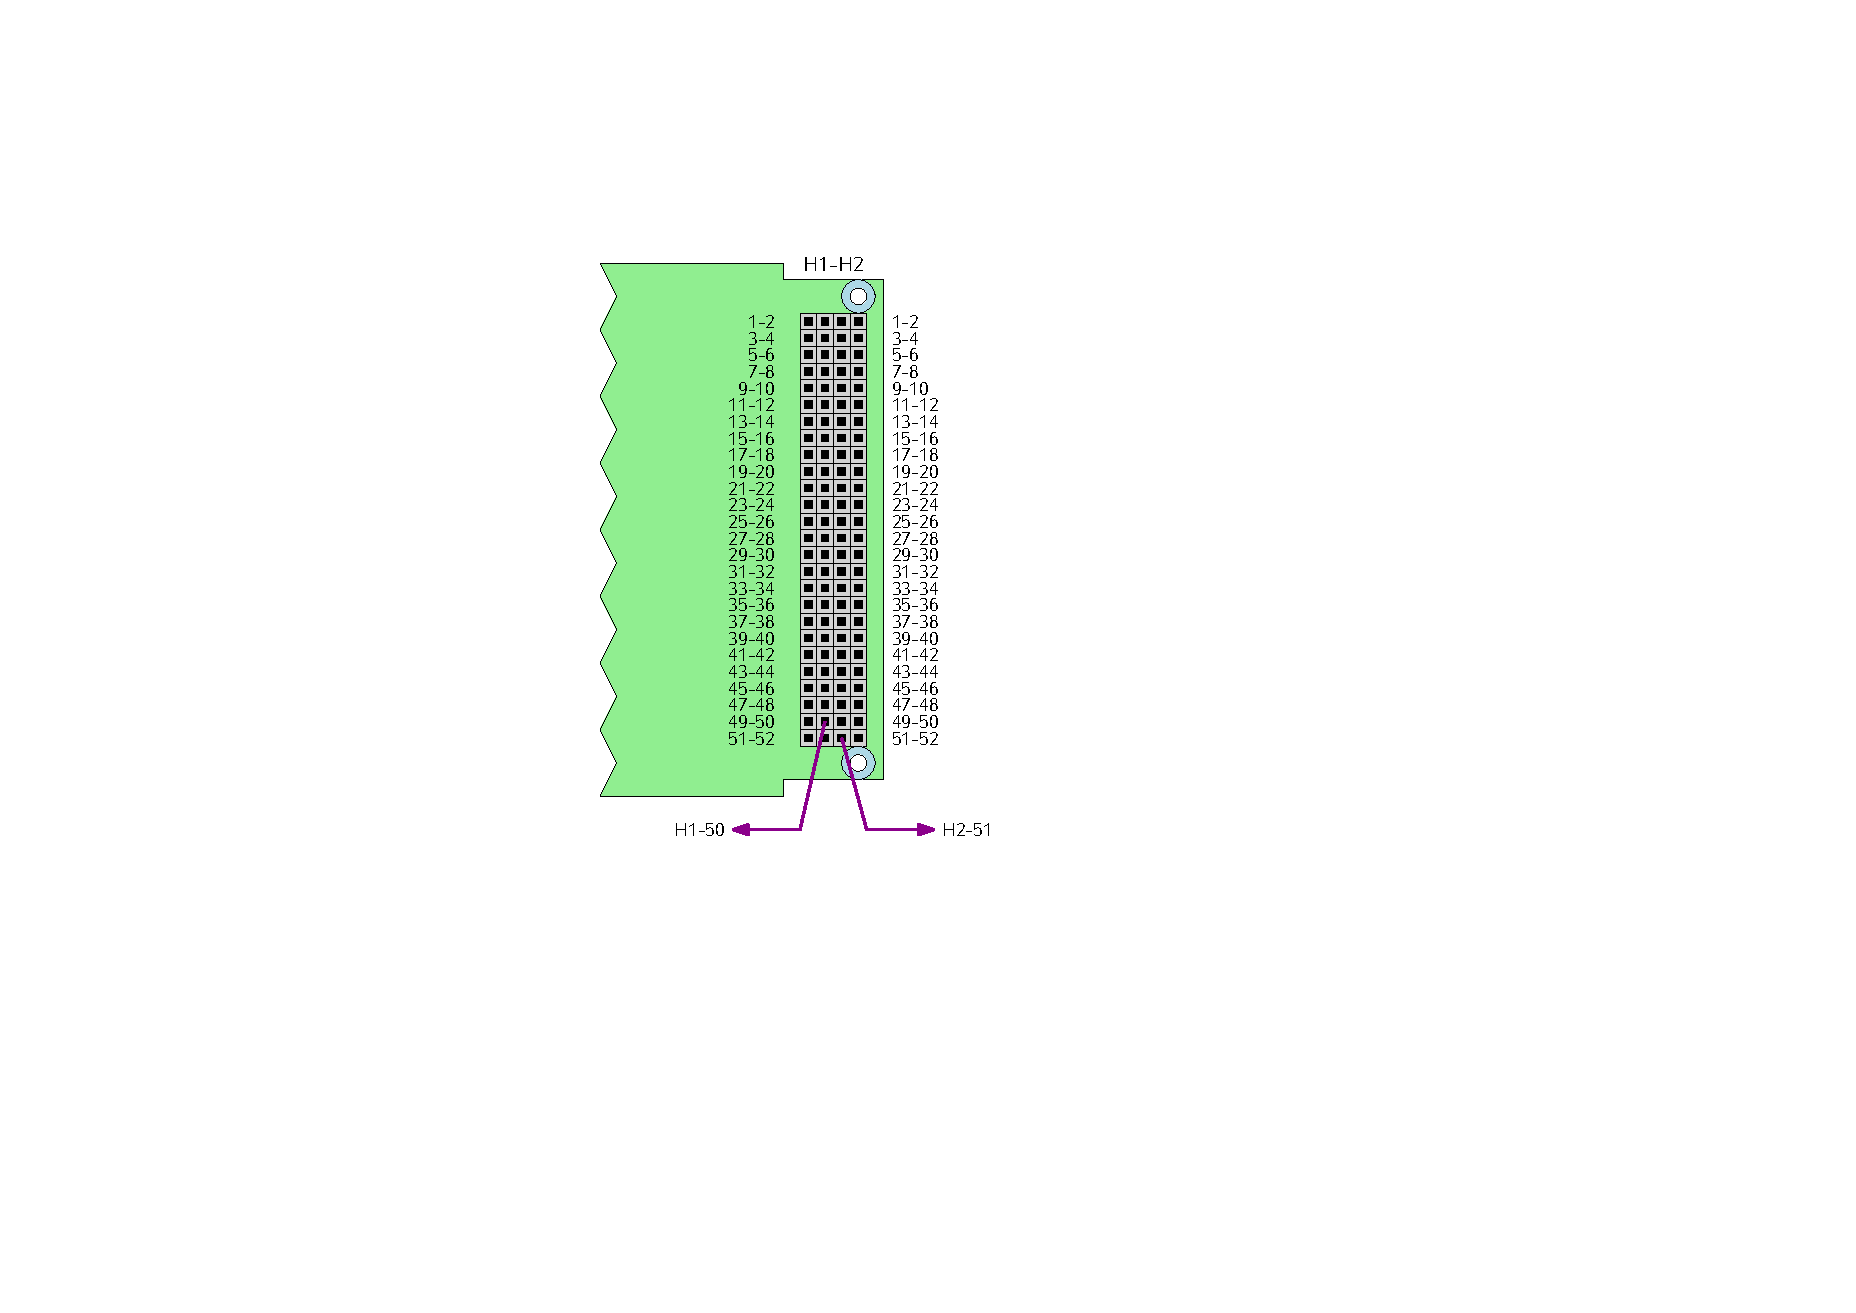
\includegraphics[width=0.5\textwidth]{figures/pc104-diagram}
        \label{fig:pc104-diagram}
        \caption{Reference diagram of the PC-104 bus.}
    \end{center}
\end{figure}

\begin{table}[!h]
    \centering
    \begin{tabular}{cllll}
        \toprule[1.5pt]
        \textit{Pin [A-B]} & \textit{H1A}     & \textit{H1B}     & \textit{H2A}  & \textit{H2B}  \\
        \midrule
        1-2                & -                & -                & -             & -             \\
        3-4                & -                & -                & -             & -             \\
        5-6                & -                & -                & UART\_RX      & -             \\
        7-8                & -                & -                & UART\_TX      & -             \\
        9-10               & -                & EN\_PWR\_5       & -             & -             \\
        11-12              & -                & EN\_PWR\_6       & -             & -             \\
        13-14              & -                & -                & -             & -             \\
        15-16              & -                & -                & -             & -             \\
        17-18              & -                & -                & -             & -             \\
        19-20              & -                & -                & -             & -             \\
        21-22              & -                & -                & -             & -             \\
        23-24              & -                & -                & -             & -             \\
        25-26              & -                & -                & PWR\_4\_5V    & PWR\_4\_5V    \\
        27-28              & -                & -                & PWR\_7\_3V3   & PWR\_7\_3V3   \\
        29-30              & GND              & GND              & GND           & GND           \\
        31-32              & GND              & GND              & GND           & GND           \\
        33-34              & -                & -                & -             & -             \\
        35-36              & -                & -                & PWR\_1\_3V3   & PWR\_1\_3V3   \\
        37-38              & -                & -                & -             & -             \\
        39-40              & -                & -                & -             & -             \\
        41-42              & -                & -                & -             & -             \\
        43-44              & -                & -                & -             & -             \\
        45-46              & PWR\_2\_3V3      & PWR\_2\_3V3      & PWR\_3\_BAT   & PWR\_3\_BAT   \\
        47-48              & PWR\_4\_5V       & PWR\_4\_5V       & -             & -             \\
        49-50              & PWR\_5\_5V       & PWR\_5\_5V       & I2C\_SDA      & -             \\
        51-52              & PWR\_6\_6V       & PWR\_6\_6V       & I2C\_SCL      & -             \\
        \bottomrule[1.5pt]
    \end{tabular}
    \caption{PC-104 connector pinout.}
    \label{tab:pc104-pins}
\end{table}

\begin{table}[!h]
    \centering
    \begin{tabular}{lL{0.29\textwidth}L{0.47\textwidth}}
        \toprule[1.5pt]
        \textbf{Signal}  & \textbf{Pin(s)}            & \textbf{Description} \\
        \midrule
        GND              & H1-29, H1-30, H1-31, H1-32, H2-29, H2-30, H2-31, H2-32 & Ground reference \\
        PWR\_1\_3V3      & H2-35, H2-36               & Power bus 1, 3.3 V, 2 A max. \\
        PWR\_2\_3V3      & H1-45, H1-46               & Power bus 2, 3.3 V, 1 A max. \\
        PWR\_3\_BAT      & H2-45, H2-46               & Power bus 3, battery terminals (+) \\
        PWR\_4\_5V       & H1-47, H1-48, H2-25, H2-26 & Power bus 4, 5 V, 3 A max. \\
        PWR\_5\_5V       & H1-49, H1-50               & Power bus 5, 5 V, 5 A max. \\
        PWR\_6\_6V       & H1-51, H1-52               & Power bus 6, 6 V, 5 A max. \\
        PWR\_7\_3V3      & H2-27, H2-28               & Power bus 7, 3.3 V, 2 A max. \\
        I2C\_SDA         & H2-49                      & Primary communication bus (data signal) \\
        I2C\_SCL         & H2-51                      & Primary communication bus (clock signal) \\
        UART\_RX         & H2-5                       & Secondary communication bus (RX) \\
        UART\_TX         & H2-7                       & Secondary communication bus (TX) \\
        EN\_PWR\_5       & H1-10                      & Enable signal of the power bus 5 \\
        EN\_PWR\_6       & H1-12                      & Enable signal of the power bus 6 \\
        \bottomrule[1.5pt]
    \end{tabular}
    \caption{PC-104 bus signal description.}
    \label{tab:pc104-signals}
\end{table}

\subsection{Solar Panels}

\subsection{Kill-Switches}

\subsection{Battery Charge}

\subsection{Remove Before Flight}

\subsection{RTDs}

\subsection{Battery Module}

\subsection{Battery Heater}
